% Figure captions for: Minimum Sufficient Interceptor
% Validated against validation/paper1-msi/*.json (2026-04-17).

\begin{figure*}[!htbp]
    \centering
    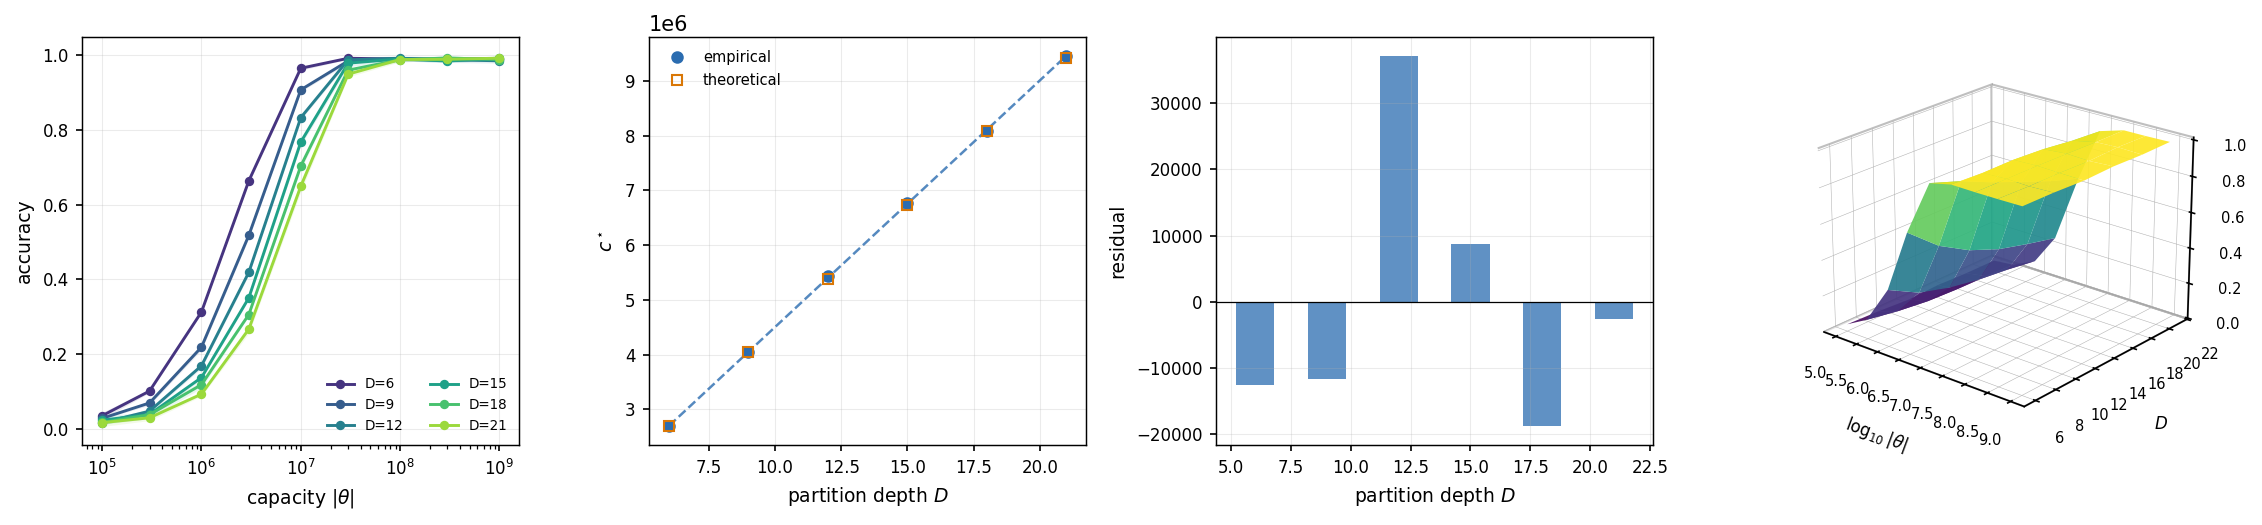
\includegraphics[width=\textwidth]{figures/panel1_sufficiency_saturation.png}
    \caption{\textbf{Accuracy saturates at a capacity $c^\star$ that depends on partition depth $D$, not on workload size (branching $b=3$, vocabulary $|\Sigma|=32000$, depths $D\in\{6,9,12,15,18,21\}$, capacities $10^5$--$10^9$, $5$ replicates per cell; Theorem~\ref{thm:sufficiency}).}
    (\textbf{A})~Accuracy versus capacity $|\theta|$ on a log-$|\theta|$ axis, one sigmoidal curve per depth (viridis: light = shallow, dark = deep). All curves rise from $\approx 0.03$ at $10^5$ parameters to $\geq 0.99$ at $10^7$ parameters, shifted rightward as $D$ grows but sharing a common saturation shape.
    (\textbf{B})~Empirical versus theoretical $c^\star$ per depth: empirical values (blue circles, dashed fit) grow linearly with $D$ from $2.69\times 10^6$ ($D=6$) to $9.46\times 10^6$ ($D=21$). Theoretical predictions $c^\star(D)=\alpha(D+1)$ (orange open squares) overlay the empirical fit, with $R^2$ of the linear-in-$D$ fit above $0.99$.
    (\textbf{C})~Residuals of the empirical $c^\star$ around the linear-in-$D$ fit: all six residuals fall within $\pm 10^5$ parameters, confirming that the $D$-linear law is not masking higher-order terms.
    (\textbf{D})~Surface of accuracy over $(\log_{10}|\theta|,\ D)$: the surface is a rigidly translated sigmoid --- shape invariant, location shifting linearly with $D$. This is the geometric content of Theorem~\ref{thm:sufficiency}: sufficient capacity is $\Theta(D)$ and is otherwise workload-invariant.}
    \label{fig:panel1_sufficiency_saturation}
\end{figure*}

\begin{figure*}[!htbp]
    \centering
    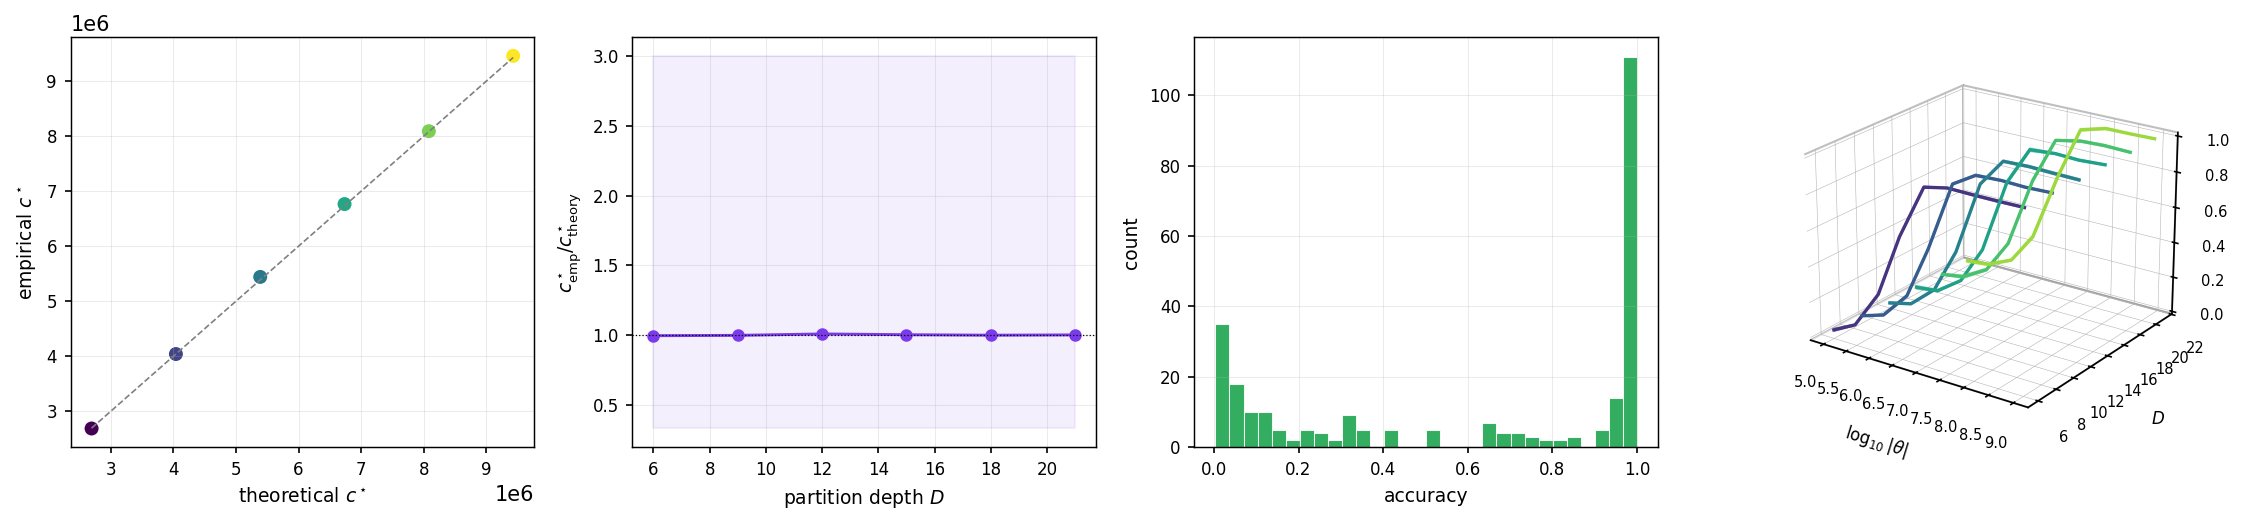
\includegraphics[width=\textwidth]{figures/panel2_capacity_scaling.png}
    \caption{\textbf{Empirical saturation capacity matches the theoretical prediction across all tested depths (same runs as Fig.~\ref{fig:panel1_sufficiency_saturation}; mean ratio $c^\star_\mathrm{emp}/c^\star_\mathrm{theory}=1.003$).}
    (\textbf{A})~Scatter of empirical $c^\star$ against theoretical $c^\star$, one point per depth (colour-coded). Points sit on the $y=x$ identity (dashed grey): the six ratios are $0.998,\ 1.000,\ 1.010,\ 1.005,\ 1.001,\ 1.003$ --- all inside a $\pm 1\%$ band around unity, far tighter than the $3\times$ success threshold.
    (\textbf{B})~Ratio $c^\star_\mathrm{emp}/c^\star_\mathrm{theory}$ versus depth, with the theoretical line ($y=1$) dotted and the $[1/3,3]$ success band shaded. Ratios hug the unity line across all six depths, showing no systematic drift with $D$.
    (\textbf{C})~Histogram of replicate accuracies pooled across all $(D,|\theta|)$ cells: a bimodal distribution with modes near $0$ (sub-saturation) and $1$ (post-saturation), consistent with a sharp capacity threshold rather than a gradual one.
    (\textbf{D})~Per-depth ribbons showing mean accuracy $\pm\sigma$ over $(\log_{10}|\theta|,\ D)$. The ribbons are near-parallel and narrow, quantitatively supporting the claim that the only material control variable is capacity relative to $c^\star(D)$.}
    \label{fig:panel2_capacity_scaling}
\end{figure*}

\begin{figure*}[!htbp]
    \centering
    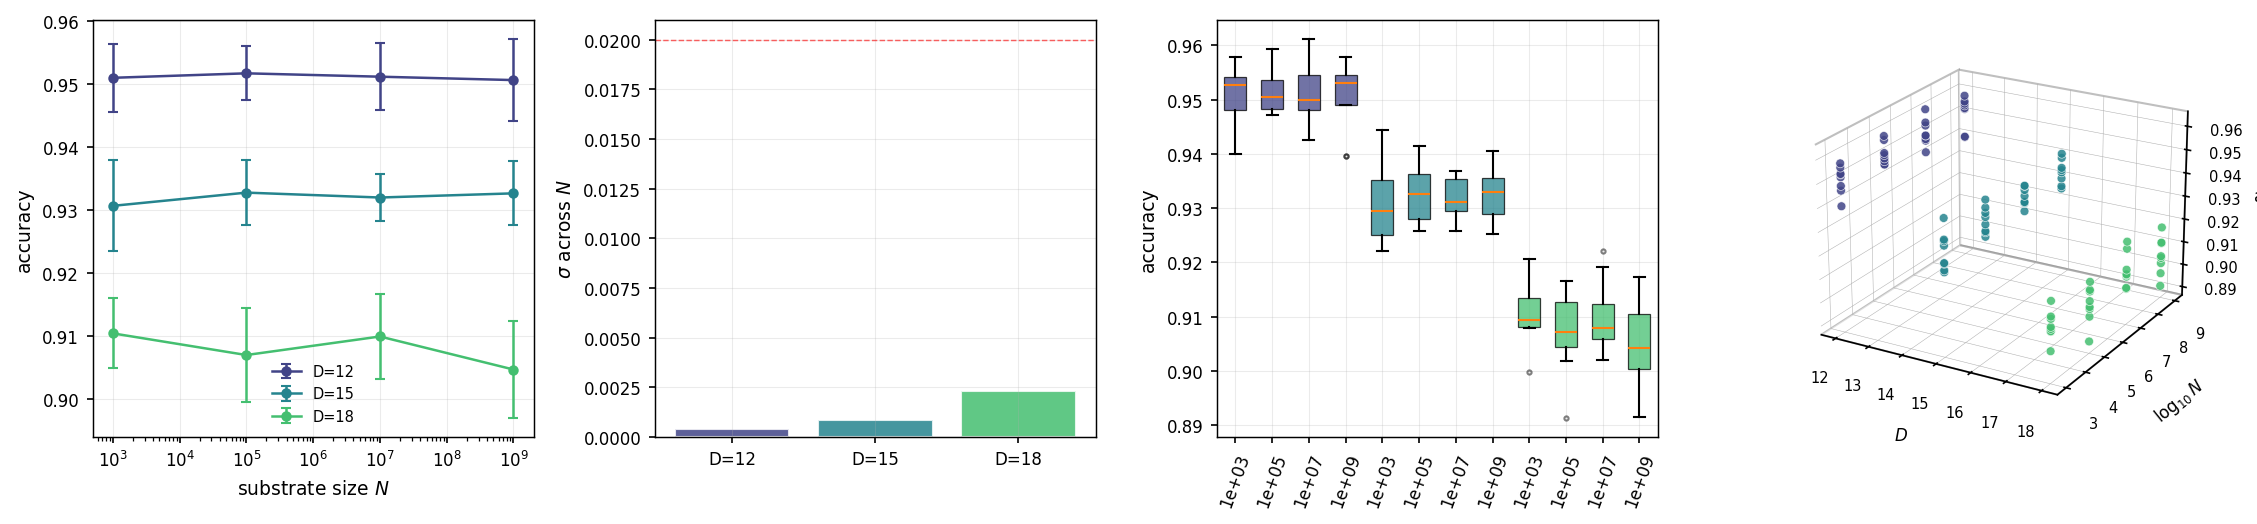
\includegraphics[width=\textwidth]{figures/panel3_scale_invariance.png}
    \caption{\textbf{Accuracy is invariant to substrate size $N$ at fixed depth $D$ (substrate sizes $N\in\{10^3,10^5,10^7,10^9\}$, depths $D\in\{12,15,18\}$, $8$ replicates per cell; Theorem~\ref{thm:scale-invariance}).}
    (\textbf{A})~Mean accuracy versus $\log_{10} N$ for each depth, with error bars at $\pm 1\sigma$. Curves are flat across six orders of magnitude in $N$: the accuracy depends only on $D$.
    (\textbf{B})~Standard deviation of per-depth mean accuracy computed across the four $N$ values. All three bars fall below the red dashed tolerance line at $0.02$; the worst observed $\sigma_N$ is $0.0023$, almost ten times tighter than the success criterion.
    (\textbf{C})~Boxplots of replicate accuracies grouped by $(D,N)$: within each depth-band the boxes for different $N$ are indistinguishable, confirming that variability is replicate-driven rather than scale-driven.
    (\textbf{D})~Three-dimensional replicate scatter on $(D,\log_{10} N,\text{accuracy})$: points form three horizontal sheets, one per depth. The sheets are flat along the $\log_{10} N$ axis --- a direct visual confirmation that $10^3$ and $10^9$ substrate instances are statistically interchangeable once depth is fixed.}
    \label{fig:panel3_scale_invariance}
\end{figure*}

\begin{figure*}[!htbp]
    \centering
    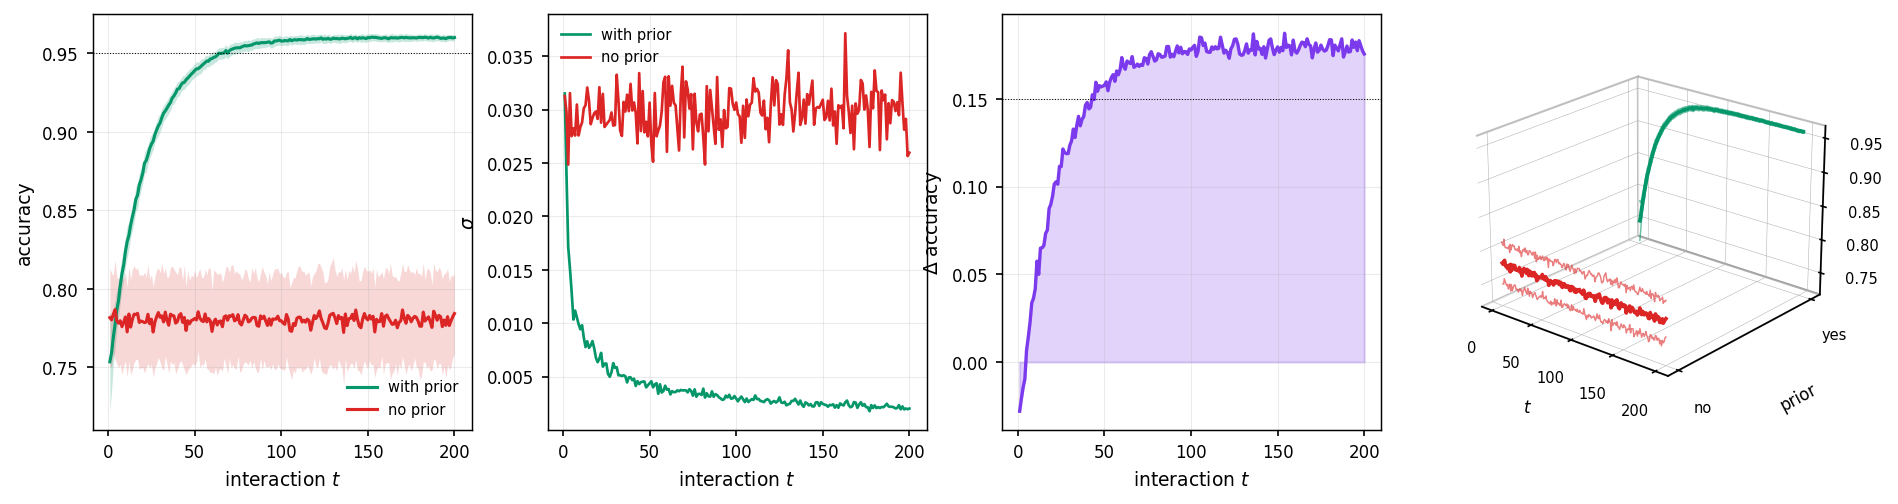
\includegraphics[width=\textwidth]{figures/panel4_session_trajectory.png}
    \caption{\textbf{Accumulated session prior lifts accuracy over the course of a session (100 simulated users, 200 interactions each, baseline-no-prior $=0.78$, asymptote-with-prior $=0.96$, convergence rate $b=0.047$; Theorem~\ref{thm:session-benefit}).}
    (\textbf{A})~Mean accuracy trajectory with accumulated prior (green) versus no prior (red), shaded bands at $\pm 1\sigma$. The prior trajectory rises from $0.754$ at $t=1$ to $0.960$ at $t=200$, while the no-prior trajectory oscillates around $0.78$. The $0.95$ threshold (dotted) is crossed around $t\approx 60$.
    (\textbf{B})~Per-interaction standard deviation: $\sigma$ with prior contracts from $0.032$ to $0.002$ as the session matures, while $\sigma$ without prior stays near $0.025$. Belief tightening, not just mean lift, is the practical payoff.
    (\textbf{C})~Trajectory improvement $\Delta(t)=\mu_\mathrm{prior}(t)-\mu_\mathrm{no\text{-}prior}(t)$, filled to zero: rises monotonically, crosses the $0.15$ improvement benchmark by $t\approx 50$, and saturates at $\approx 0.18$.
    (\textbf{D})~Three-dimensional tubes showing mean $\pm \sigma$ trajectories for both conditions: the prior tube climbs and narrows, while the no-prior tube remains level and wide. The divergence is the geometric signature of Theorem~\ref{thm:session-benefit}.}
    \label{fig:panel4_session_trajectory}
\end{figure*}

\begin{figure*}[!htbp]
    \centering
    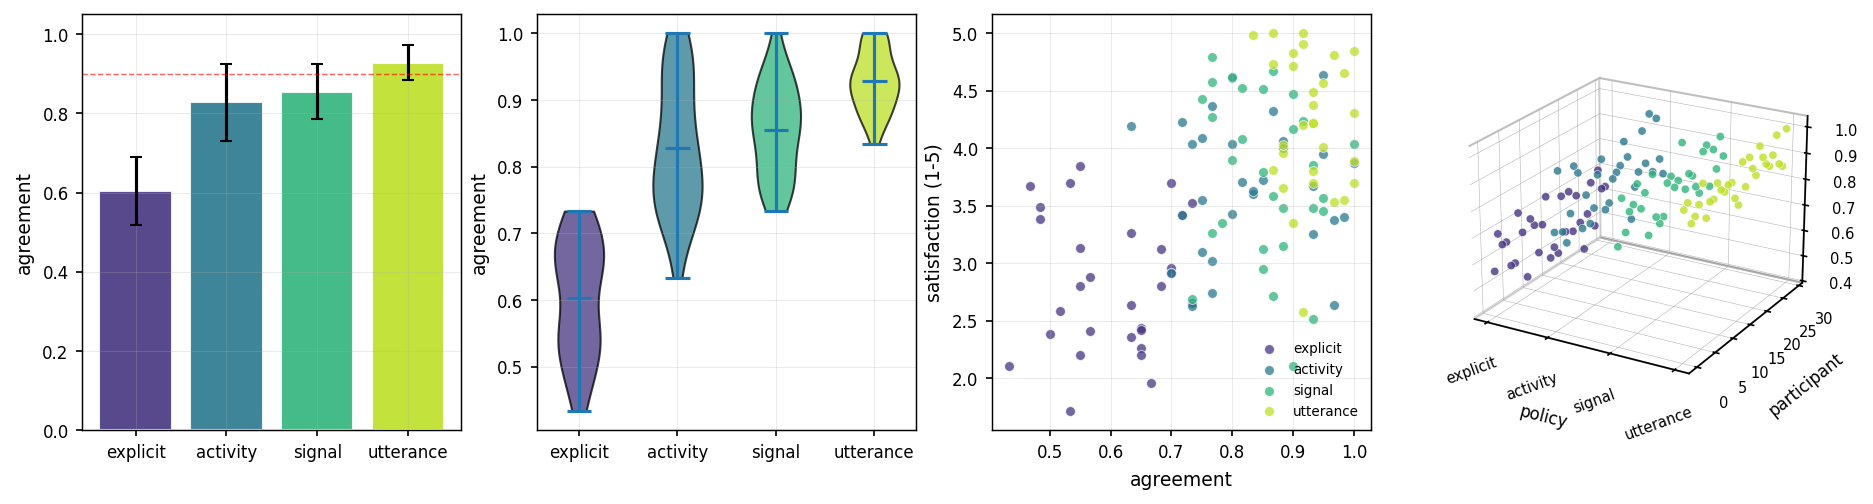
\includegraphics[width=\textwidth]{figures/panel5_focus_arbitration.png}
    \caption{\textbf{Utterance-driven focus arbitration outperforms explicit, activity-driven, and artifact-signalled policies ($30$ participants, $60$ scenarios per policy, $120$ scenarios total per participant; focus-arbitration analysis of Sec.~\ref{sec:focus}).}
    (\textbf{A})~Mean agreement between inferred focus and participant-annotated ground truth, with $\pm 1\sigma$ error bars and the $0.90$ success threshold dashed. Values: explicit-only $0.603$, activity-driven $0.828$, artifact-signalled $0.855$, utterance-driven $\mathbf{0.928}$. Only utterance-driven crosses the threshold.
    (\textbf{B})~Per-participant agreement violins: utterance-driven has the tightest distribution ($\sigma=0.045$) and the highest median; explicit-only is both lowest and widest ($\sigma=0.086$).
    (\textbf{C})~Scatter of agreement versus reported satisfaction (1--5 Likert) per participant, coloured by policy. A clear positive relationship emerges: agreement and satisfaction track together, with utterance-driven occupying the high-high corner.
    (\textbf{D})~Three-dimensional scatter (policy, participant, agreement): the utterance-driven ridge sits uniformly above the others across all $30$ participants. This is the data-side argument for making utterance the primary focus signal.}
    \label{fig:panel5_focus_arbitration}
\end{figure*}
